\chapter{Governing parameters of  fluid-elastic galloping}
\label{chap:goven_para}

\section{Introduction}

This chapter contains the formulation of non dimensional governing parameters namely, the combined mass-stiffness \massstiff \ and the combined mass-damping \massdamp \ and the results and discussion demonstrating the influence of them. These parameters are formulated by obtaining the relevant time-scales of the system followed by non-dimesnionlising the governing QSS oscillator equation.  

A comparison of Quasi-steady state data presented using the classical VIV parameters and the newly formulated \massstiff \ and \massdamp is presented and it is concluded that \massdamp provides a better collapse for velocity amplitude and mean power compared the classical reduced velocity (\ustar) particularly because unlike \ustar, \massdamp \ does not include a frequency component in it. This is followed by the presentation of QSS data and discussion on the influence of \massstiff \ and \massdamp \ on power, which concludes that the power transfer is a primary function of \massdamp \ and a weak function of \massstiff.

Following this, a comparison of the QSS data with Direct Numerical Simulations (DNS) is presented. This reveals that the power transfer of the DNS data is strongly influenced by both \massstiff \ and \massdamp. Further analysis reveals that there is a good agreement between QSS and DNS for velocity and power at substantially high \massstiff\. As \massstiff \ decreases, the deviation (between QSS simulations and DNS) increases. Power spectral analysis of the DNS data shows a significant response at the vortex shedding at low \massstiff. The relative strength was found out to be an inverse function of \massstiff, which provides a clear explanation for the deviation between QSS simulations and DNS data at low \massstiff. This is primarily due to the influence of vortex shedding where this effect is not accounted in the QSS model.


\section{Formulation of the non-dimensionalised parameters \massstiff \ and \massdamp }
\label{sec: pi_1,pi_2_formulation}

The natural time scales of the system could be obtained by linearising the quasi-steady equation of motion. (Eq:\KJ{equation of motion}) and finding the eigenvalues. The non-linear terms of the forcing function are truncated and the equation of motion could be expressed as, 

\begin{equation}
\label{eqn:eom_linear}
m\ddot{y}{+}c\dot{y}{+}ky{=}\frac{1}{2}\rho U^2 \mathcal{A} a_1\left(\frac{\dot{y}}{U}\right),
\end{equation}

After combining the $\dot{y}$ terms and solving for eigenvalues the following solutions for the eigenvalues could be obtained. 

 \begin{equation}
 \label{eqn:eigs}
 \lambda_{1,2}= -\frac{1}{2}\frac{c-\frac{1}{2}\rho U\mathcal{A}a_1}{m}\pm\frac{1}{2}\sqrt{\left[\frac{c-\frac{1}{2}\rho U\mathcal{A}a_1}{(m)}\right]^2-4\frac{k}{m}}.
 \end{equation} 
 
 Galloping essentially occurs at low frequencies therefore it can be assumed that the spring is relevantly weak and therefore, $k \rightarrow 0$. Hence a single non-zero eigenvalue remains which is, 
  
  \begin{equation}
  \label{eqn:eigs_nospring}
  \lambda=-\frac{c-\frac{1}{2}\rho U\mathcal{A}a_1}{m}.
  \end{equation}
  
  Further, if it is assumed that the mechanical damping is weaker than the fluid dynamic forces on the body the non zero eigenvalue could be further simplified to,
  
 \begin{equation}
 \label{eqn:eigs_nospring_nodamp}
 \lambda=\frac{\frac{1}{2}\rho U\mathcal{A}a_1}{m}.
 \end{equation}  

In this representation $\lambda$ represents the inverse time scale of the motion of the body due to the effect of long-time fluid dynamic forces (or forced due to the induced velocity). This term could also be re-written and $\lambda$ could be expressed as 

\begin{equation}
\label{eqn:timescale}
\lambda = \frac{a_1}{m^*}\frac{U}{D}
\end{equation}

This form clearly shows the significant parameters that influences the inverse time scale of the system. $\partial C_Y / \partial \alpha $, the rate of change in the fluid dynamic force on the body, with respect to the induced angle of attack, is represented by $a_1$. $\frac{U}{D}$ represents the inverse advective time scale of the incoming flow, and the mass ratio is resented by \mstar. Increasing $a_1$ would result in a rapid change of the fluid dynamic force with a small change of the induced angle $\theta$, which is proportional to transverse velocity $\dot{y}$. It can be seen in equation \ref{eqn:timescale} that an increase of $a_{1}$ would result in an increase of the inverse time scale or decrease the response time of the body. In contrast the mass ratio has the opposite effect where an increase in \mstar will lead to a decrease in $\lambda$, since a heavier body (or a body with higher inertia) would have a slower response. 

In order to find the relevant dimensionless groups of the problem, the time scale formulated could be used to non-dimensionalise the equation of motion. The equation of motion presented in Equation \KJ{put final equation of motion} can be non-dimensionalised using the non dimensional time $\tau$, defined as $\tau=t(a_1/m^*)(U/D)$. The non-dimensional equation of motion could then be represented as, 

 \begin{equation}
 \label{eqn:eom_nondim}
 \ddot{Y} + \frac{m^{*2}}{a_1^2}\frac{kD^2}{mU^2}Y = \left(\frac{1}{2} - \frac{m^*}{a_1}\frac{cD}{mU}\right)\dot{Y} - \frac{a_1A_3}{m^{*2}}\dot{Y}^3 + \frac{a_1^3a_5}{m^{*4}}\dot{Y}^5 - \frac{a_1^5a_7}{m^{*6}}\dot{Y}^7.
 \end{equation}
 
 The equation could be further altered by regrouping the coefficients into non-dimenasional groups and could be expressed as, 
 
  \begin{equation}
  \label{eqn:eom_nondim_regroup}
  \ddot{Y} + \frac{4\pi^{2}m^{*2}}{U^{*2}a_1^2}Y = \left(\frac{1}{2} - \frac{c^*m^*}{a_1}\right)\dot{Y} - \frac{a_1A_3}{m^{*2}}\dot{Y}^3 + \frac{a_1^3a_5}{m^{*4}}\dot{Y}^5 - \frac{a_1^5a_7}{m^{*6}}\dot{Y}^7,
  \end{equation}  

\ustar is the reduced velocity which is the typical independent variable ussed in vortex-induced vibration studies. \cstar is the non-dimensional damping parameter which is expressed as $c^*=cD/mU$. 

By analysing equation \ref{eqn:eom_nondim_regroup} it is clear that five dimensionless parameters play a role in setting the response of the system. These are namely the stiffness, damping, mass ratio, the geometry and the Reynolds number. The stiffness is repented by the reduced velocity \ustar, the damping by \cstar and the mass ratio by \mstar. The geometry and the Reynolds number are represented by the coefficients $a_n$, of the polynomial fit to the $C_y$ curve. Using the natural time scales of the system, grouping of these non-dimensional parameters into two groups in the non-dimensional equation of motion, suggests that there are two groups that governs the response which are: $\Gamma_1 = 4\pi^2m^{*2}/U^{*2}a_1^2$ and $\Gamma_2 = c^*m^*/a_1$. $\Gamma_1$ could be described as a combined mass-stiffness, where $\Gamma_2$ could be expressed as a combined mass-damping parameter for a given geometry and a Reynolds number. It is assumed that the stiffness plays a minor role, $\Gamma_2$ seems more likely parameter to collapse the data. The wind tunnel data in the classic paper of galloping by \citep{Parkinson1964} adopted a parameter similar to $\Gamma_2$ to collapse the data. 

All of the quantities that formulate $\Gamma_1$ and $\Gamma_2$ except $a_1$ in theory, could be obtained before an experiment. However in order to obtain the value of $a_1$ static body experiments are required making it relatively difficult to obtain. Here, the \reynoldsnumber and the geometry remains constant and therefore multiplying $\Gamma_1$ with ${a_1}^2$ and $\Gamma_2$ with $a_1$ suitable parameters could be obtained, and formulate a mass-stiffness parameter $\massstiff =  4\pi^2m^{*2}/U^{*2}$, and a mass-damping parameter defined as $\massdamp = c^*m^*$. Therefore equation \ref{eqn:eom_nondim_regroup} can be written in terms of \massstiff \ and \massdamp. 

  \begin{equation}
  \label{eqn:eom_nondim_regroup_pi_1_pi_2}
  \ddot{Y} + \massstiff Y = \massdamp \dot{Y} - \frac{a_1a_3}{m^{*2}}\dot{Y}^3 + \frac{a_1^3a_5}{m^{*4}}\dot{Y}^5 - \frac{a_1^5a_7}{m^{*6}}\dot{Y}^7,
  \end{equation} 
  
From equation \ref{eqn:eom_nondim_regroup_pi_1_pi_2}, it is clear that the governing parameters of the non dimensionlised equation are \massstiff \ \massdamp and \mstar. However, form closer inspection it is possible to see that \mstar has an impact on the non-linear terms of the forcing function. The velocity pf the and hence the induced angle of attack needs to be very high in order for the non-linear terms to be applicable. 

\section{Quasi-steady state results}
\label{sec:qss_results} 

\subsection{Classical VIV parameters vs. \massstiff \ and \massdamp.}
\label{subsec:compare_data}


Vortex-induced vibrations being another form fluid-structure interaction which occurs in a slender structure, has been investigated as candidate for power extraction from external flows. Significant progress on this problem have been made by \cite{Bernitsas2008a-concept,Bernitsas2009,Raghavan2010a,Lee2011b} and other colleagues in VIVCACE group in the University of Michigan. Hence, it may seem that it is reasonable to present the data in a fluid-elastic problem using the same parameters in a VIV problem.

\begin{figure}
  \setlength{\unitlength}{\textwidth}
  \fbox{
  \begin{picture}(1,0.9)(0,0)
    % % %90
      % % % Parkinson Data 
      \put(0.035,0.5){\includegraphics[width=0.5\unitlength]{../FnP/gnuplot/displacement_amp_re200.eps}}
      \put(0.035,0.27){\includegraphics[width=0.5\unitlength]{../FnP/gnuplot/velocity_amp_re200.eps}}
      \put(0.035,0.02){\includegraphics[width=0.5\unitlength]{../FnP/gnuplot/mean_power_re_200.eps}}
      
      \put(0.495,0.27){\includegraphics[width=0.5\unitlength]{../FnP/gnuplot/velocity_amp_collapsed_re200.eps}} 
      \put(0.495,0.02){\includegraphics[width=0.5\unitlength]{../FnP/gnuplot/mean_power_collapsed_re_200.eps}}
      \put(0.495,0.5){\includegraphics[width=0.5\unitlength]{../FnP/gnuplot/displacement_amp_collpased_re200.eps}}
      
%      \put(0.23,0.00){ $\displaystyle\frac{c}{\rho\mathcal{A}U}$}
%      \put(0.73,0.00){ $\displaystyle\frac{c}{\rho\mathcal{A}U}$}

      \put(0.28,0.00){\ustar}
      \put(0.78,0.00){\massdamp}
      
      \put(0.01,0.405){$\displaystyle\frac{V}{D}$}\
       \put(0.01,0.63){$\displaystyle\frac{A}{D}$}
      
      \put(-0.02,0.13){$\displaystyle\small\frac{P_{m}}{\rho \mathcal{A}U^3 }$}
      
      \put(0.093,0.705){\small(a)}
      \put(0.555,0.705){\small(b)}
      \put(0.093,0.475){\small(c)}
      \put(0.555,0.475){\small(d)}
      \put(0.093,0.225){\small(e)}
      \put(0.555,0.225){\small(f)}

  \end{picture}
}
  \caption{Displacement amplitude, velocity amplitude and mean power data as functions of two different independent varibles. Data presented in (a), (c) and (e) using the classical VIV parameter $\ustar$, obtained at $Re=200$ and $m^*=20$ at three different damping ratios: $\zeta=0.075$ ($\times$), $\zeta=0.1$ (\ding{117}) and $\zeta=0.15$ (+). (b) (d) and (f)  are the same data presented using the combined mass-damping parameter (\massdamp) as the independent variable.  }
  \label{fig:compare_data}
\end{figure}

QSS data presented in figure \ref{fig:compare_data} at $\reynoldsnumber=200$, shows a comparison between classical VIV and the newly formulated parameters presented as independent variables. The displacement amplitude, velocity amplitude and the mean power is presented in sub-figures (a), (c) and (e), as functions of the classical VIV parameter \ustar for different $\zeta$. The same data as functions of \massdamp, are presented in sub-figures (b), (d) and (f), for various, reasonably high values of \massstiff \KJ{put the parameters used section}. Sub-figure (e) shows a similar trend to \cite{Barrero-Gil2010a}. The Value of the peak power remains constant. However, the power curve shifts to the right as $\zeta$ is increased. Here, in figure \ref{fig:compare_data} the maximum dimensionless power is achieved at two times the velocity at which the galloping starts, which is similar to the observations made by \citet{Barrero-Gil2010a,vicente-Ludlam2014}. An excellent collapse for velocity amplitude and mean power could be observed on the data, presented using the dimensionless group \massdamp, formulated using the natural time scales of the system. This implies that essentially velocity amplitude and the mean power is dictated by \massdamp which furthermore, implies that the natural frequency of the system which is used to scale \ustar, $\zeta$ and \massstiff does not have a significant influence on the behaviour of the system, unlike VIV, which is a resonant phenomenon.  
 

\subsection{High and low \reynoldsnumber \ data}
\label{subsec:high_Re_data}

% !TeX spellcheck = en_GB
\begin{figure}
  \setlength{\unitlength}{\textwidth}

        \begin{picture}(1,0.3)(-0.02,0)

      % % % Parkinson Data 
%      \put(0.025,0.5){\includegraphics[width=0.5\unitlength]{../FnP/gnuplot/displacement_amp_collapsed_parkinson.eps}}
%      \put(0.025,0.27){\includegraphics[width=0.5\unitlength]{../FnP/gnuplot/velocity_amp_collapsed_parkinson.eps}}
%      \put(0.495,0.27){\includegraphics[width=0.5\unitlength]{../FnP/gnuplot/velocity_amp_collapsed_re200.eps}}
      
      \put(0.025,0.02){\includegraphics[width=0.5\unitlength]{../FnP/gnuplot/mean_power_collapsed_parkinson.eps}}
      \put(0.495,0.02){\includegraphics[width=0.5\unitlength]{../FnP/gnuplot/mean_power_optimum_re_200.eps}}
%      \put(0.495,0.5){\includegraphics[width=0.5\unitlength]{../FnP/gnuplot/displacement_amp_collpased_re200.eps}}
      
%      \put(0.23,0.00){ $\displaystyle\frac{c}{\rho\mathcal{A}U}$}
%      \put(0.73,0.00){ $\displaystyle\frac{c}{\rho\mathcal{A}U}$}

      \put(0.28,0.00){\massdamp}
      \put(0.74,0.00){\massdamp}
      
     
       \put(-0.03,0.13){$\displaystyle\frac{P_{m}}{\rho \mathcal{A}U^3 }$}
      

      \put(0.095,0.218){\small(a)}
      \put(0.565,0.218){\small(b)}
      
    \end{picture}

  \caption{Mean power as a function of \massdamp. Data presented at (a) $\reynoldsnumber=22300$, $\massstiff=200$ ($\times$), $massstiff=2000$ (\ding{117}) and $\massstiff=10000$ (+). (b) $\reynoldsnumber=200$, $\massstiff=100$. Hysteresis could be observed at high \reynoldsnumber  }
    \label{fig:collapsed_data}
\end{figure}

 %vspace{10cm}


The successful collapse of data, mean power in particular using \massdamp for low Reynolds number ($\reynoldsnumber=200$), could be replicated at high Reynolds numbers. An example case is presented in figure \ref{fig:compare_data} at $\reynoldsnumber=22300$ for selected vales of \massstiff. The successful collapse of mean power data at high Reynolds numbers shows that suitability of using \massdamp \ as an independent variable across a large range of Reynolds numbers. 

Hysteresis is evident in the high Reynolds number case ($\reynoldsnumber=22300$). Manipulating the initial condition (initial displacement) lead to obtaining different solutions for the same \massdamp \ value. The upper and lower branch were obtained by giving an initial displacement which was higher than the expected amplitude and providing a lower initial displacement respectively. Even though in theory, there is a possibility of a third state, this unstable branch could not be achieved with a time integration method (also observed by \citep{Vio2007}) such as the one employed in this study.

\subsection{Dependence on mass-stiffness, \massstiff}
\label{subsec:dependence pi_1}

\begin{figure}
  \setlength{\unitlength}{\textwidth}
\fbox{
        \begin{picture}(1,1.1)(0,0.35)

      % % % Parkinson Data 
      \put(0.09,1.1){\includegraphics[width=0.757\unitlength]{../FnP/gnuplot/displacement_high_pi_1.eps}}
      \put(0.1,0.75){\includegraphics[width=0.75\unitlength]{../FnP/gnuplot/velocity_high_pi_1.eps}}
      \put(0.1,0.35){\includegraphics[width=0.75\unitlength]{../FnP/gnuplot/mean_power_high_pi_1.eps}}
      
         \put(0.07,0.95){$\displaystyle\frac{V}{D}$}\
         \put(0.07,1.3){$\displaystyle\frac{A}{D}$}
         \put(0.05,0.6){$\displaystyle\frac{P_{m}}{\rho \mathcal{A}U^3 }$}



%      
%      \put(0.45,0.7){\small(a)}
%      \put(0.926,0.7){\small(b)}
%      \put(0.726,0.45){\small(c)}
%  

      
    \end{picture}
}
  \caption{QSS data at high \massstiff \ levels. (a) displacement amplitude, (b) velocity amplitude and (c) mean power as a function of \massdamp. Data presented at four different combined mass-stiffness levels.\ $\massstiff=10 \ (\mstar=20,\ \ustar \approx 40)$ \ (\ding{117}),\ $\massstiff=100 \ (\mstar=130,\ \ustar \approx 80) \ (+)$ and \ $\massstiff=1000 \ (\mstar=400,\ \ustar \approx 40) \ (\triangle)$}
    \label{fig:high_pi_1}
\end{figure}

 %vspace{10cm}


From the results of sections \ref{subsec:compare_data} and \ref{subsec:high_Re_data} shows essentially a single variable governs the mean extracted power, which is the combined mass-damping parameter, \massdamp. The time scale analysis carried out in  section \ref{sec: pi_1,pi_2_formulation} shows that not only \massdamp \ but also \massstiff influences the system. Previous studies such as \cite{bouclin:77} have also reported a complex interaction between the displacement amplitude and the natural frequency, for high natural frequencies in particular; or in this instance equivalent to low values of \massstiff.  This section investigates the impact of \massstiff further. The overall behavior of the system is divided into two regimes, one for ``high" \massstiff \ and the other for ``low" \massstiff and analysed.

The mean power as a function of \massdamp \ for a range of values of \massstiff is presented in figure \ref{fig:high_pi_1}. In the two subfigures presented, (a) shows the data for $\massstiff \geq 10$, while (b) shows data for $\massstiff \leq 10$.  The excellent collapse in figure \ref{fig:high_pi_1}(a) shows that for $\massstiff \geq 10$, the mean power is independent of \massstiff.

In contrast figure \ref{fig:high_pi_1}(b) shows that for low values of $\massstiff \leq 10$, the predicted mean power increases as \massdamp \ decreases. This indicates that at this region ($\massstiff < 10$), the mean power is a weak function of \massstiff; hence, providing a distinction between high and low regimes of \massstiff. The mean extracted power is only a function of \massdamp \ where $\massstiff \geq 10$ or for high \massstiff. For low values, $\massstiff < 10$, the mean power becomes a strong function of \massdamp \ and a weak function of \massstiff.

It is clear that regardless of the value of \massstiff, the variation of power with \massdamp \ is essentially the same. As \massdamp \ is increased, the mean extracted power will increase to the point which, it will attain some maximum value and then decrease. This relationship between power and \massdamp \ could be explained by analysing the time histories of selected cases. 
AS an example, data at $\massstiff=10$, $m^*=20$ and $\reynoldsnumber=200$ are presented in figure \ref{fig:power_time_histories}. Three major regions where the value of the power curve are considered. These regions are \massdamp\ less than (region 1), equal to (region 2) and greater than (region 3) to the \massdamp\ value where the mean power is at its maximum.

\begin{figure}

  \setlength{\unitlength}{\textwidth}
%  \fbox{
  \begin{picture}(1,0.58)(0,0.35)
    % % % 90
    \put(0.03,0.76){\includegraphics[width=0.35\unitlength]{../FnP/gnuplot/power_time_history_015.eps}}
    \put(0.03,.58){\includegraphics[width=0.35\unitlength]{../FnP/gnuplot/f_y_history_015.eps}}
    \put(0.03,0.4){\includegraphics[width=0.35\unitlength]{../FnP/gnuplot/theta_time_history_015.eps}}
    
    % % 165
    \put(0.36,0.76){\includegraphics[width=0.35\unitlength]{../FnP/gnuplot/power_time_history_54.eps}}
    \put(0.36,.58){\includegraphics[width=0.35\unitlength]{../FnP/gnuplot/f_y_history_54.eps}}
    \put(0.36,0.4){\includegraphics[width=0.35\unitlength]{../FnP/gnuplot/theta_time_history_54.eps}}
    
    \put(0.68,0.76){\includegraphics[width=0.35\unitlength]{../FnP/gnuplot/power_time_history_08.eps}}
    \put(0.68,.58){\includegraphics[width=0.35\unitlength]{../FnP/gnuplot/f_y_history_08.eps}}
    \put(0.68,0.4){\includegraphics[width=0.35\unitlength]{../FnP/gnuplot/theta_time_history_08.eps}}
    
    \put(0.55,0.36){$\displaystyle{\frac{tU}{D}}$}
    \put(0.2,0.36){$\displaystyle{\frac{tU}{D}}$}
    \put(0.85,0.36){$\displaystyle{\frac{tU}{D}}$}
    
    \put(0.0,0.87){$\frac{P}{\rho \mathcal{A}U^3}$}
    \put(0.01,0.66){$F_y$}
    \put(0.01,0.49){$\theta$}
    
    \put(0.08,0.76){(a)}
    \put(0.08,0.58){(d)}
    \put(0.08,0.38){(g)}
    
    \put(0.4,0.76){(b)}
    \put(0.4,0.58){(e)}
    \put(0.4,0.38){(h)}
    
    \put(0.72,0.76){(c)}
    \put(0.72,0.58){(f)}
    \put(0.72,0.38){(i)}
  \end{picture}
%}
  \caption{Time histories of $P_t$, $P_d$, $F_y$ and $\theta$ at $\massdamp=0.15$, $0.54$ and $0.8$ from the QSS model. Data was obtained at $m^*=20$, $\massstiff=10$ and \reynoldsnumber=200. The time histories of $P_t$ ( \solidrule[4mm]\hspace{1mm}) and $P_d$ (\protect\dashedrule) are presented for: (a) $\massdamp= 0.15$; (b) $\massdamp= 0.54$; (c) $\massdamp= 0.8$. Time histories of the instantaneous force $F_y$ for: (d) $\massdamp= 0.15$; (e) $\massdamp= 0.54$; (f) $\massdamp= 0.8$. Time histories of the instantaneous angle $\theta$ for: (g) $\massdamp= 0.15$; (h) $\massdamp= 0.55$; (i) $\massdamp= 0.8$.}
  \label{fig:power_time_histories}
\end{figure}






The damping is low is low in region 1 ($\massdamp=0.15$) in comparison with region 2 and 3. Although this may lead to larger oscillations, according to equation \ref{eqn:power} damping is required to dissipate and therefore extract power. Hence, a low mean power output is gained at low damping. The high velocity amplitude leads the equivalent incident angle $\theta$ to exceed the positive range of $C_y$ (i.e. $0<\theta<6^\circ$ as shown in figure\ref{cy ploynomial}(a)) resulting a negative dissipated power by damping $P_d$ over some portion of the cycle as shown in figure \ref{fig:power_time_histories} (a). The galloping force $F_y$ and the transverse velocity $\dot{y}$ are not in phase in this portion of the cycle where the force opposes the direction of travel. As a consequence, during this period of time the opposite of what is expected happens, where the power is transferred from the structure to the fluid. Since \massdamp \ is substantially low, from an energy perspective, the mechanical damping is not sufficient to remove the energy transferred from the fluid to the structure through work during other times of the cycle. Hence, as depicted by the negative region of $P_d$, this excess energy is transferred back to the fluid.



A clear sinusoidal signal of both $P_d$ and $P_t$ (\ref{fig:power_time_histories}(c)) could be observed at region 3 where $\massdamp=0.8$ and the damping constant is high. The equivalent incident angle $\theta$ (which for small values, is proportional to the transverse velocity of the body) is in phase with the galloping force $F_y$ as shown in figures \ref{fig:power_time_histories}(f) and  \ref{fig:power_time_histories}(i). The velocity amplitude is small in this case resulting $\theta$ falling within the rage where the fluid-dynamic force ($F_y$) increases within the incident angle (i.e. $0<\theta \leq 5^\circ$ as shown in figure \ref{fig:lift_curves}(a)). These conditions are favourable for high power output according to equation \ref{power_alt}. Be that as it may, in this case the velocity is limited because of the high damping resulting relativity low fluid dynamic forcing. 

A harmony between the high and low values of damping could be found at region 2  ( $\massdamp=0.54$). It is evident that $P_d$ remains periodic but is not a pure sinusoidal signal. Two `peaks' are present in a single half cycle from the time history graph of $P_d$ as shown in figure \ref{fig:power_time_histories}(b). The velocity amplitude actually exceeds the equivalent incident angle where the fluid-dynamic forces peaks (i.e. $\theta=5^\circ$ in \ref{cy ploynomial} (a)) in this scenario. The dip in between the two peaks in a single half cycle correspond approximately to the time where the transverse velocity is higher that 0.09 and $F_y$ is decreasing with increasing transverse velocity. As this region is the best compromise between region 1 and region 3, the maximum mean power could be attained in this region. Region 2 could also be identified as the ``sweet spot" for energy extraction as the damping is high enough to obtained a high power output while not so high for the motion to be completely suppressed. 


\subsection{Dependence on the mass ratio \mstar}
\label{sec:chp-pi_1_pi2_mstar}


 










    


